\PassOptionsToPackage{pdftex}{graphicx}
\documentclass[sigconf,9pt,natbib=false]{acmart}

% begin packages
% ==============
\usepackage[utf8]{inputenc}
\usepackage[T1]{fontenc}
% \usepackage[pdftex]{graphicx}
\graphicspath{{./images/}{./plots/}}
\DeclareGraphicsExtensions{.pdf,.jpeg,.png}
\usepackage{amsmath}
\usepackage{url}
\usepackage[inline]{enumitem}
\usepackage{todonotes}
\usepackage{caption}
\usepackage{subcaption}
\pagenumbering{gobble}
\usepackage[newfloat]{minted}
\SetupFloatingEnvironment{listing}{name=List.,within=none}
\captionsetup[table]{justification=centerlast,
                     labelsep=newline,
                     font=sf,
                     textfont=footnotesize}
\usepackage{booktabs}
\usepackage{xcolor}
\usepackage[detect-weight=true,detect-family=true,binary-units=true,list-units=single,range-units=single]{siunitx}
\usepackage[nolist]{acronym}
\begin{acronym}
  \acro{CPS}{Cyber-Physical System}
  \acro{NCS}{Networked Control System}
  \acroindefinite{NCS}{an}{a}
  \acro{LAN}{Local-Area Network}
  \acro{WLAN}{Wireless Local-Area Network}
  \acro{KPI}{Key Performance Indicator}
  \acro{WPAN}{Wireless Personal Area Network}
  \acro{CSMA/CD}{Carrier-Sense Multiple Access with Collision Detection}
  \acro{CLEAVE}{ControL bEnchmArking serVice on the Edge}
  \acro{OS}{Operating System}
  \acro{UDP}{User Datagram Protocol}
  \acro{TCP}{Transmission Control Protocol}
  \acro{RMS}{Root Mean Square}
  \acro{RTT}{Round-Trip Time}
  \acro{CI}{Confidence Interval}
  \acro{AP}{Access Point}
  \acro{API}{Application Programming Interface}
  \acro{SSF}{Swedish Foundation for Strategic Research}
  \acro{TECoSA}{Trustworthy Edge Computing Systems and Applications}
  \acro{ABC}{Abstract Base Class}
  \acroplural{ABC}[ABCs]{Abstract Base Classes}
\end{acronym}

% references
% \usepackage[
%   style=numeric-comp,
%   sorting=none,
%   sortcites,
%   hyperref,
%   mincitenames=1,
%   maxcitenames=2,
%   maxbibnames=2,
%   minbibnames=1,
%   citestyle=numeric-comp, % for [1, 2] instead of [1], [2]
%   backend=bibtex
% ]{biblatex}
% \bibliography{bibliography.bib}
% \AtBeginBibliography{\small}
% \AtEveryBibitem{\clearfield{day}}
% \AtEveryBibitem{\clearfield{isbn}}
% \AtEveryBibitem{\clearfield{url}}
% \AtEveryBibitem{\clearfield{series}}
% \AtEveryBibitem{\clearlist{location}}
% \AtEveryBibitem{\clearfield{doi}}

% for dealing with ACM's stupid bibtex requirements
% \usepackage{biblatex2bibitem}
\usepackage[nosort,compress]{cite}

\usepackage{orcidlink}
\usepackage[all]{hypcap}
\usepackage[capitalize,nameinlink,noabbrev]{cleveref}
% \crefname{subfigure}{Subfigure}{Subfigures}
% \Crefname{subfigure}{Subfigure}{Subfigures}
\crefname{listing}{Listing}{Listings}
\Crefname{listing}{Listing}{Listings}

\hypersetup{
  hidelinks,
  colorlinks=true,
  allcolors=black,
  pdfstartview=Fit,
  breaklinks=true
}

\title[CLEAVE]{CLEAVE:\@ Scalable and Edge-Native Benchmarking of\\{Networked Control Systems}}

%authorlist
\author{Manuel {Olguín Muñoz}}
\orcid{0000-0002-3383-2335}
\email{molguin@kth.se}
\affiliation{%
\institution{KTH Royal Institute of Technology}%
% \department[0]{Division of Information Science and Engineering}%
% \department[1]{School of EECS}%
\city{Stockholm}%
\country{Sweden}%
}

\author{Neelabhro Roy}
\orcid{0000-0002-5777-7780}
\email{nroy@kth.se}
\affiliation{%
\institution{KTH Royal Institute of Technology}%
% \department[0]{Division of Information Science and Engineering}%
% \department[1]{School of EECS}%
\city{Stockholm}%
\country{Sweden}%
}

\author{James Gross}
\orcid{0000-0001-6682-6559}
\email{jamesgr@kth.se}
\affiliation{%
\institution{KTH Royal Institute of Technology}%
% \department[0]{Division of Information Science and Engineering}%
% \department[1]{School of EECS}%
\city{Stockholm}%
\country{Sweden}%
}

% top matter
% \acmConference[EdgeSys'22]{}{}{}  % TODO
\settopmatter{printacmref=true, printccs=true, printfolios=true}
\setcopyright{none}

\begin{CCSXML}
<ccs2012>
    <concept>
        <concept_id>10003033.10003079.10003082</concept_id>
        <concept_desc>Networks~Network experimentation</concept_desc>
        <concept_significance>300</concept_significance>
        </concept>
    <concept>
        <concept_id>10003033.10003079.10011672</concept_id>
        <concept_desc>Networks~Network performance analysis</concept_desc>
        <concept_significance>300</concept_significance>
        </concept>
    <concept>
        <concept_id>10002944.10011123.10010912</concept_id>
        <concept_desc>General and reference~Empirical studies</concept_desc>
        <concept_significance>300</concept_significance>
        </concept>
    <concept>
        <concept_id>10002944.10011123.10010916</concept_id>
        <concept_desc>General and reference~Measurement</concept_desc>
        <concept_significance>300</concept_significance>
        </concept>
    <concept>
        <concept_id>10002944.10011123.10011131</concept_id>
        <concept_desc>General and reference~Experimentation</concept_desc>
        <concept_significance>500</concept_significance>
        </concept>
    <concept>
        <concept_id>10002944.10011123.10011130</concept_id>
        <concept_desc>General and reference~Evaluation</concept_desc>
        <concept_significance>300</concept_significance>
        </concept>
    <concept>
        <concept_id>10002944.10011123.10011674</concept_id>
        <concept_desc>General and reference~Performance</concept_desc>
        <concept_significance>500</concept_significance>
        </concept>
    <concept>
        <concept_id>10010520.10010553.10010559</concept_id>
        <concept_desc>Computer systems organization~Sensors and actuators</concept_desc>
        <concept_significance>500</concept_significance>
        </concept>
    <concept>
        <concept_id>10010520.10010553.10010554.10010556</concept_id>
        <concept_desc>Computer systems organization~Robotic control</concept_desc>
        <concept_significance>100</concept_significance>
        </concept>
    <concept>
        <concept_id>10010520.10010521.10010537.10003100</concept_id>
        <concept_desc>Computer systems organization~Cloud computing</concept_desc>
        <concept_significance>300</concept_significance>
        </concept>
    <concept>
        <concept_id>10010520.10010521.10010537.10010538</concept_id>
        <concept_desc>Computer systems organization~Client-server architectures</concept_desc>
        <concept_significance>300</concept_significance>
        </concept>
  </ccs2012>
\end{CCSXML}

\ccsdesc[300]{Networks~Network experimentation}
\ccsdesc[300]{Networks~Network performance analysis}
\ccsdesc[300]{General and reference~Empirical studies}
\ccsdesc[300]{General and reference~Measurement}
\ccsdesc[500]{General and reference~Experimentation}
\ccsdesc[300]{General and reference~Evaluation}
\ccsdesc[500]{General and reference~Performance}
\ccsdesc[500]{Computer systems organization~Sensors and actuators}
\ccsdesc[100]{Computer systems organization~Robotic control}
\ccsdesc[300]{Computer systems organization~Cloud computing}
\ccsdesc[300]{Computer systems organization~Client-server architectures}

\copyrightyear{2022} 
\acmYear{2022} 
\setcopyright{rightsretained} 
\acmConference[EdgeSys'22]{5th International Workshop on Edge Systems, Analytics and Networking }{April 5--8, 2022}{RENNES, France}
\acmBooktitle{5th International Workshop on Edge Systems, Analytics and Networking (EdgeSys'22), April 5--8, 2022, RENNES, France}\acmDOI{10.1145/3517206.3526272}
\acmISBN{978-1-4503-9253-2/22/04}

%Benchmarking human-in-the-loop applications is complex.
%This limits reproducibility as well as feasibility of performance evaluations.
%In this paper we present EdgeDroid, a benchmarking suite that addresses these challenges.
%Our core idea rests on recording traces of these applications \jjw{-> application traces} which are then replayed out \jjw{remove out} in a controlled fashion based on an underlying model of human behavior \jjw{-> emulating human behaviors}.
%The traces are then exposed to the original backend compute process of the respective human-in-the-loop application, generating realistic feedback.
%This allows for an automated system that greatly simplifies benchmarking large scale scenarios.
%Our results confirm the utility of EdgeDroid as a tool for system designers, application developers and researchers.

%\jjw{Alternative version:
Many emerging mobile applications, including \acs{AR} and \acs{WCA}, aim to provide seamless user interaction.
However, the complexity of benchmarking these human-in-the-loop applications limits reproducibility and makes performance evaluation difficult.
In this paper, we present EdgeDroid, a benchmarking suite designed to reproducibly evaluate these applications.

Our core idea rests on recording traces of user interaction, which are then replayed at benchmarking time in a controlled fashion based on an underlying model of human behavior. 
This allows for an automated system that greatly simplifies benchmarking large scale scenarios and stress testing the application.
Our results show the benefits of EdgeDroid as a tool for both system designers and application developers.
%}



\begin{document}
\maketitle
\renewcommand{\shortauthors}{{Olguín Muñoz} et al.}

\section{Introduction}\label{sec:intro}

\gls{WCA} applications are a novel category of wearable, edge-native applications aiming to amplify human cognition in both daily activities and professional settings.
These systems aim to seamlessly integrate into the day-to-day of users, leveraging compute-intensive algorithms to analyze user and environment information and provide real-time, context-aware information and feedback.
\gls{WCA} applications originally emerged as assistive use-cases for individuals suffering from cognitive decline due to aging or traumatic brain injuries~\cite{satyanarayanan2009case,ha2014towards,satyanarayanan2019augmenting}, and have since expanded to a greater range of use cases.
In particular, following the success of non-wearable \gls{XR} and cognitive assistance in industrial settings~\cite{funk2015cognitive,wang2022comprehensive}, there is increasing interest in the research community in the application of \gls{WCA} for step-by-step assistance for complex assembly tasks~\cite{chen2017empirical,belletier2021wearable}.

A defining characteristic of these applications is their lack of reliance on intentional user inputs to trigger responses.
They are intended to operate as autonomous guides, much akin to how \gls{GPS} systems guide drivers, tracking their progress and providing feedback and instructions at appropriate times.
This context-sensitivity and proactivity in providing user feedback translate into a reliance on high-dimensional, complex, unstructured inputs, such as real-time video, which require intensive compute capabilities to process.
This also translates into latency-sensitivity, as with any \gls{AR} application.
Delays and jitter can be jarring to the user, causing discomfort and leading them to make mistakes and potentially even abandoning the application altogether.
On the other hand, as their name suggests, these systems are by design \emph{wearable}, which implies the use of lightweight, battery-powered, low energy consumption devices.

The combination of these opposing characteristics has led to \gls{WCA} applications being identified in the literature as prime candidates for offloading to the edge~\cite{ha2014towards,chen2017empirical,chen2018application}.
However, many unknowns still remain before consumer-scale adoption of these applications can become a reality.
One key gap in knowledge pertains to the current lack of tools and methodologies for scalable and repeatable study of \gls{WCA} application performance and resource utilization in realistic deployments.
Due to their human-in-the-loop nature, these applications present a challenge to benchmark and characterize, in particular in real-scale deployments where dozens or even hundreds of users might concurrently use the system.
Accordingly, recruiting a  cohort of subjects for realistic benchmarking and study of \gls{WCA} systems can be prohibitively cumbersome and expensive for many research groups and system designers
There exists therefore a real need for scalable tools for \gls{WCA} benchmarking which do not rely on direct testing of the human-in-the-loop.

\medskip

In that context, the contributions of this paper are:
\begin{enumerate}
    \item\label{item:contrib:model} We introduce the first, to our knowledge, stochastic model for human timings in \gls{WCA} applications.
    Using the data collected for~\cite{olguinmunoz2021impact} as a base, we build a stochastic model which takes as input past measurements of system responsiveness and produces realistic step execution times.
    We also introduce a novel way to generate dynamic traces of frames for \gls{WCA} applications which can be combined with the timing model for a full end-to-end emulation of a human.
    We name this new model \emph{\edgedroid}; a direct, more realistic evolution of our initial EdgeDroid approach~\cite{olguinmunoz2018demoscaling,olguinmunoz2019edgedroid}.
    \item\label{item:contrib:footprint} Using this model, we study the implications of realistic human behavior for the \emph{application lifetime footprint} of \gls{WCA}, understanding this term as the duration of a specific complete execution of the application task.
    In accordance with previous work~\cite{olguinmunoz2021impact}, we find dependencies between system responsiveness and human step execution times that lead to substantially different application lifetimes when compared to a first-order baseline which does not take into account human behavior.
    \item\label{item:contrib:optimization} Finally, we study the potential for optimization in \gls{WCA} when considering human behavior using our model.
    We develop a generic model for the stochastic optimization of resource consumption versus responsiveness trade-offs in these applications, which we apply to two potential avenues for \gls{WCA} optimization; number of processed samples and energy consumption per step.
    First, we study the potential for reducing the number of samples captured per step.
    This is a valuable endeavor, as reducing the number of samples captured and subsequently processed directly translates in lower bandwidth demand on the wireless network and processor time demand on the cloudlet.
    Next, we explore the potential for direct optimization of energy consumption.
    The economic feasibility of WCA, and hence its likelihood of commercial adoption depends on it not being a resource hog, and this work furthers that effort.
    Leveraging our more involved user model, combined with the introduced optimization approach, we achieve a \textasciitilde\SI{60}{\percent} reduction in the number of samples processed per step.
    We also achieve an improvement of \SI{20}{\percent} in energy consumption, all while maintaining comparable levels of system responsiveness.
\end{enumerate}

\medskip

This paper is structured as follows.
\cref{sec:relwork} discusses related work in the field of \gls{WCA} modeling.
In \cref{sec:background} we define and discuss key concepts in \gls{WCA}, as well as summarize the key conclusions from our previous work relating to the relationship between system responsiveness and human behavior in these applications~\cite{olguinmunoz2021impact}.
In \cref{sec:model} we detail our model for the generation of realistic human timing in \gls{WCA}.
We present its design, verify its expected behavior with respect to our previous results, and introduce the dynamic trace generation for full end-to-end emulation of human behavior.
Next, in \cref{sec:implications:footprint}, we discuss the potential implications of such a model on application lifetimes by studying a small series of representative scenarios.
This is followed by a more in-depth investigation in \cref{sec:implications:optimization} on the potential consequences of a human timing model on the general optimization of \gls{WCA} systems.
In the same section, we introduce our generic optimization framework for resource consumption versus responsiveness trade-offs in \gls{WCA}.
Finally, in \cref{sec:conclusion} we summarize and conclude this paper, as well as briefly discuss potential avenues for future work.

\section{The \gls{CLEAVE} framework}\label{sec:approach}

In this section, we detail our \gls{CLEAVE} framework for the performance evaluation of \glspl{NCS}, with an emphasis on edge deployments.
Our design follows a virtualized emulation approach; providing a framework for the real-time \emph{emulation} of physical control systems and the easy implementation of softwarized controllers interacting with \emph{real} networks.
\gls{CLEAVE} is thus a platform with an easy-to-use \gls{API} on which a multitude of \gls{NCS} types can be emulated.
This allows for great flexibility, as the core components of the \gls{NCS} can be switched out while maintaining the realism of the network, the most complex and limiting component of edge \glspl{NCS}.

The framework is distributed as \emph{free and open-source} software through the \emph{GitHub} organization of the \emph{KTH ExPECA} research group\footnote{\url{https://github.com/KTH-EXPECA/CLEAVE}}.
We also plan to provide a library of \gls{NCS} implementations, making the tool even more accessible.

\subsection{Design and Implementation}\label{sec:design}

The design of \gls{CLEAVE} attempts to target a broad a set of different control systems as possible, and tries to minimize the number of assumptions made about the systems implemented on top of the framework.
These are:
\begin{enumerate}
    \item Controllers can be stateful or stateless, but they exclusively control a single plant.
    \item Plants and controllers interact in a ``request-response'' manner.
    We currently don't support setups in which the controller generates an actuation command without there first being a request from the plant.
    \item Controller and plant communicate over a TCP/IP network.
    \item The physical state behavior of the plant can be implemented in a discrete-time manner.
    \item Values associated to sensors and actuators can be represented as integers, floating point numbers, booleans, or sequences of bytes.
    \item A plant has zero or more sensors attached to it, with potentially different sampling rates.
    \item A plant has zero or more actuators attached to it.
\end{enumerate}

\cref{fig:cleave:ncs:struct} shows an overview of the conceptual structure and operation of \gls{CLEAVE}.
The \emph{State} implements the discrete-time behavior of the Plant.
At the beginning of each time-step, actuated variables in the \emph{State} are updated with values obtained from the \emph{Actuator} objects.
Conversely, at the end of each time-step, sensed variables are sampled and used to update values associated with \emph{Sensor} objects.
These values are processed at the \emph{Sensors} (e.g.\ to add noise) before being sent over the network to the \emph{Controller}.
The \emph{Controller} calculates actuation values and updates the \emph{Actuators} over the network.
Finally, the \emph{Actuators} process the actuation values and hold the results until they are read at the next time-step.

Implementation-wise, \gls{CLEAVE} is built on top of the well-established and stable \emph{Twisted}\footnote{\url{https://twistedmatrix.com}} asynchronous programming and networking framework.
The aforementioned core components (\emph{State}, \emph{Controller}, \emph{Sensors}, and \emph{Actuators}) are provided as \glspl{ABC} with core functionality that users must extend for their specific use cases and \glspl{NCS}.
The framework makes no assumptions about the inner workings of the user implementations of these classes other than the interfaces they expose.
Users are therefore free to implement arbitrarily complex functionality in these components.
On the other hand, \gls{CLEAVE} handles network communication and metric collection autonomously; users only need to select the desired transport protocol (we do however provide an \gls{API} for extending the available transports).

Below we present a brief overview of the design and implementation of the core components.

%\begin{description}[style=nextline]
%\begin{itemize}
\textbf{State Base Class}:
\gls{ABC} with an abstract method
\mintinline{python}{advance()} which must be extended with the implementation of discrete-time emulation of the plant.
The \mintinline{python}{advance()} method is called by the framework periodically according to the configured emulation update rate, and should perform a single time-step of the discrete-time emulation.
Two optionally extensible methods, \mintinline{python}{initialize()} and \mintinline{python}{shutdown()} are provided to implement single-fire set-up and tear-down procedures.

    % This class also provides functionality for the automatic tracking and updating of sensed and actuated values.
    % This is handled through special auxiliary classes, \emph{SensorVariable} and \emph{ActuatorVariable}, which when instantiated and assigned to an attribute of the \emph{State} allow the framework to track and modify them.

\textbf{Controller Base Class}:
Defines a single abstract method \mintinline{python}{process()}, taking a mapping of names to values corresponding to the sensed variables of the \emph{State}, and returning a similar mapping corresponding to the actuated variables.
This method is called by \gls{CLEAVE} in an event-based manner whenever samples are received from the plant side; however, we intend to extend this to time-interval-based approaches.

\textbf{Sensor Base Class}:
Implements processing of monitored stated variables before sending them over the network to the \emph{Controller}.
This base class must be initialized with a property name (corresponding to the monitored \emph{State} attribute) and a sampling rate in \si{\hertz}, and provides an abstract method \mintinline{python}{process_sample()} which must be extended with an implementation of the processing performed on each sample.

\textbf{Actuator Base Class}:
Performs the processing of actuation values obtained over the network from the \emph{Controller}.
It is initialized with a property name corresponding to the name of the actuated \emph{State} attribute, and provides two abstract methods which must be implemented by extending classes:
\begin{enumerate*}[itemjoin={{; }}, itemjoin*={{; and }}]
\item \mintinline{python}{set_value()}, called by the framework whenever a new value for the corresponding actuated attribute is received
\item \mintinline{python}{get_actuation()}, called on every time-step and must return a value to apply to the actuated attribute.
\end{enumerate*}
%\end{itemize}
%\end{description}


\subsection{Configuring and Executing \pgls{NCS}}

Once the core components for the emulation have been defined and implemented, they need to be registered with the framework.
This is done through Python scripts which define a number of required (and some optional) top-level variables, corresponding to emulation parameters such as the \emph{State}, \emph{Controller}, \emph{Sensor}, and \emph{Actuator} subclasses to use; the emulation update rate; the controller-side host and address; data output directories; \emph{et cetera}.
These Python configuration files are then provided as arguments to the \texttt{cleave} command line provided by the framework.
\gls{CLEAVE} imports and parses them, and then sets up and executes the emulation.

Although the core design of \gls{CLEAVE} follows a single-loop approach, multi-loop scenarios can be easily implemented through the combination of multiple \gls{CLEAVE} instances.
The framework does not make any assumptions about the individual components other than the signatures of methods on the \glspl{ABC} that must be extended and implemented.
Combined with the Python emulation configuration scripts, this makes development of more complex scenarios merely a matter of implementing the desired functionality within the framework itself.

\subsection{Current Implementations}

\begin{figure}
    \centering
    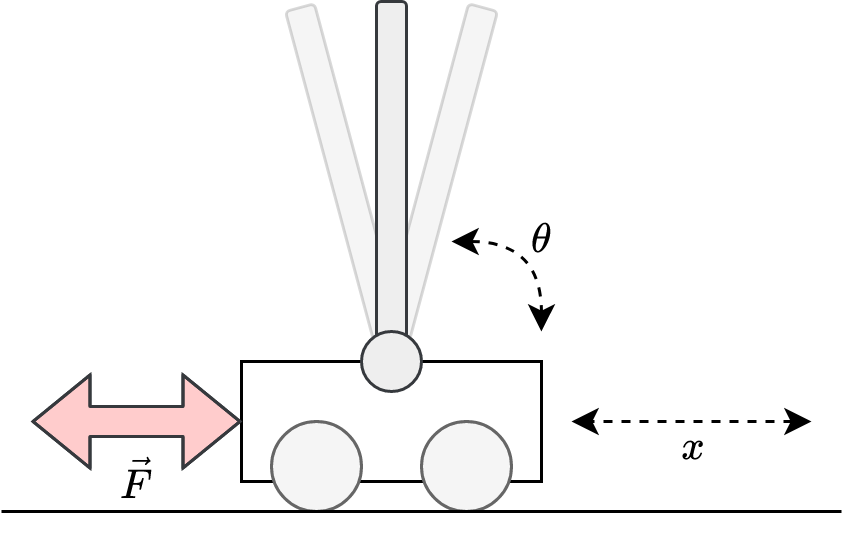
\includegraphics[width=.6\columnwidth]{publications/2022CLEAVE/images/inverted_pendulum.png}
    \caption{
        The 2D inverted pendulum system.
    }\label{fig:invpend}
\end{figure}

For the purpose of this work, we have used \gls{CLEAVE} to implement an emulated \emph{inverted pendulum} control loop (see \cref{fig:invpend}), the goal of which is to balance the vertically free-swinging pendulum by applying horizontal forces on the cart.
We have chosen this system as an initial benchmark for its relative simplicity as well as prevalence in the field of automatic control as one of the fundamental examples of linear control.

The inverted pendulum plant \emph{State} is implemented as a real-time discrete-time physical emulation using CLEAVE's API and a 2D physics library\footnote{Pymunk: \url{http://www.pymunk.org/en/latest/}}, updated at a constant \SI{120}{\hertz} (this value is configurable; in this case it corresponds to the maximum achievable stable rate on our available hardware).
\emph{Sensors} for the angle, position, angular velocity, and velocity of the \emph{State}, and an \emph{Actuator} for the horizontal force applied to the cart are implemented as ``perfect'', i.e.\ values are returned as-is, without any added noise.
For the controller side, a proportional-differential strategy is implemented using the framework \emph{Controller} API and the \emph{NumPy} numeric computation library\footnote{NumPy: \url{https://numpy.org/}}.
Plant and controller are then packaged into containers, for ease of orchestration and reparametrization, and to mimic real-world deployment.

A previously mentioned, we eventually plan to build an open library of emulated control loops.\footnote{%
    At the moment of writing, we are in the process of implementing \emph{model-predictive} as well as \emph{deep neural network} controllers for the inverted pendula plants.%
}
The inverted pendulum plant is merely a proof-of-concept, and \gls{CLEAVE} could be used to implement much more complex physical systems with even more stringent latency requirements.
For instance, the flexibility afforded by the choice of programming language and the abstractions detailed in \cref{sec:design}, allow for relatively straightforward emulation of autonomous drone dynamics.
Propeller dynamics could be implemented by \emph{Actuator} objects, gyroscopes by \emph{Sensors}, and the physical behavior of the plant could be modeled using a general purpose 3D physics engine (\emph{e.g.} the Panda3D\footnote{\url{https://docs.panda3d.org/1.10/python/programming/physics/builtin/index}{https://docs.panda3d.org/1.10/python/programming/physics/builtin/index}} engine).


\section{Use case validation}\label{sec:experiments}

In this section, we demonstrate the utility of \ac{CLEAVE} by walking readers through an example use case.
With this, we aim to showcase the ability of our framework to provide accurate and repeatable measurements of the performance of \acp{NCS} deployed on edge computing infrastructure.

We present the following use case scenario.
A simple \ac{NCS} consisting of an \emph{inverted pendulum} plant controlled by a \emph{proportional-differential} controller is to be deployed on an Edge server.
The connection between plant and server is over a WiFi (IEEE 802.11n) link.
Moreover, there are a number of video-streaming applications running concurrently on the Edge setup.

We believe this to be an interesting and representative use-case scenario for a number of reasons.
Firstly, the inverted pendulum is broadly used as a benchmark in control-system literature, see for instance\ \cite{Baumann2018LowPower} and\ \cite{Natale2004InvPendEthernet}.
A key reason for this is that such a relatively simplistic system allows for straightforward reparametrization to obtain varied system dynamics, which in turn makes a broader range of experiments possible.
Secondly, similar, albeit non-Edge-enabled, setups have been a reality in industry for almost two decades, as evidenced by\ \cite{Gupta2010NCSOverview}.
Thirdly, although real deployments would most assuredly employ mobile technologies due to the added benefits of mobility and range, the \acp{RTT} offered by these technologies are higher, or at best equal, those offered by WiFi.
4G, for instance, has average \acp{RTT} of around a few hundred milliseconds, which is orders of magnitude greater than the values measured in our scenario, and current 5G deployments offer \ac{RTT} values barely matching the sub-\SI{10}{\milli\second} values we obtain for WiFi.
Thus, we argue that using WiFi allows for more experimental freedom, as the system can be tweaked to obtain worse \acp{RTT} more akin to those of mobile technologies while still having the option to study best-case scenarios with very low-latencies.
Finally, video analytics is one of the main proposed use cases for edge computing~\cite{Ananthanarayanan2017Analytics,Yi2017Analytics,Wang2018Analytics}, and thus we foresee edge \ac{NCS} deployments being deployed in parallel with such applications in the future.
However, before deployment can become a reality, key questions such as: 
``what are the baseline requirements of the \ac{NCS}?''; ``what are the achievable best-case end-to-end latencies in the system?''; and
``how does the concurrent video-streaming traffic affect \ac{NCS} stability?'' need to be answered.

We attempt to study these questions using the experimental setup in \cref{fig:cleave:expsetup}.
\ac{CLEAVE} is deployed on a testbed consisting of \num{10} Raspberry Pi 4B  clients connected wirelessly to an IEEE 802.11n \ac{AP}.
Connected to the Ethernet backbone of this \ac{AP} is a general-purpose \verb|x86_64| desktop computer acting as a Cloudlet/Edge server.

% % Please add the following required packages to your document preamble:
% \usepackage{booktabs}
% \usepackage{graphicx}
\begin{table}[]
    \centering
    \caption{Hardware used in the experiments.}\label{tab:hardware}
    \resizebox{\columnwidth}{!}{%
    \begin{tabular}{@{}llrrrl@{}}
    \toprule
    \multicolumn{1}{c}{\textbf{}} &
      \multicolumn{1}{c}{\textbf{CPU}} &
      \multicolumn{1}{c}{\textbf{\begin{tabular}[c]{@{}c@{}}Freq\\ {[}\si{\giga\hertz}{]}\end{tabular}}} &
      \multicolumn{1}{c}{\textbf{\begin{tabular}[c]{@{}c@{}}Core\\ Count\end{tabular}}} &
      \multicolumn{1}{c}{\textbf{\begin{tabular}[c]{@{}c@{}}RAM\\ {[}\si{\giga\byte}{]}\end{tabular}}} &
      \multicolumn{1}{c}{\textbf{\begin{tabular}[c]{@{}c@{}}Operating\\ System\end{tabular}}} \\ \midrule
    \textbf{Cloudlet} &
      \begin{tabular}[c]{@{}l@{}}Intel\textregistered{} Core\texttrademark{}\\ i7-8700\end{tabular} &
      \num{3.2} &
      \num{6} &
      \num{32} &
      \begin{tabular}[c]{@{}l@{}}Ubuntu Server \\20.04 LTS \\Kernel v5.4.0\\\ \end{tabular} \\
    \textbf{Client} &
      \begin{tabular}[c]{@{}l@{}}Cortex-A72\\ (ARM v8)\end{tabular} &
      \num{2.0} &
      \num{4} &
      \num{8} &
      \begin{tabular}[c]{@{}l@{}}Ubuntu Server \\20.04 LTS \\Kernel v5.4.0\end{tabular} \\ \bottomrule
    \end{tabular}%
    }
\end{table}

\begin{figure}
    \centering
    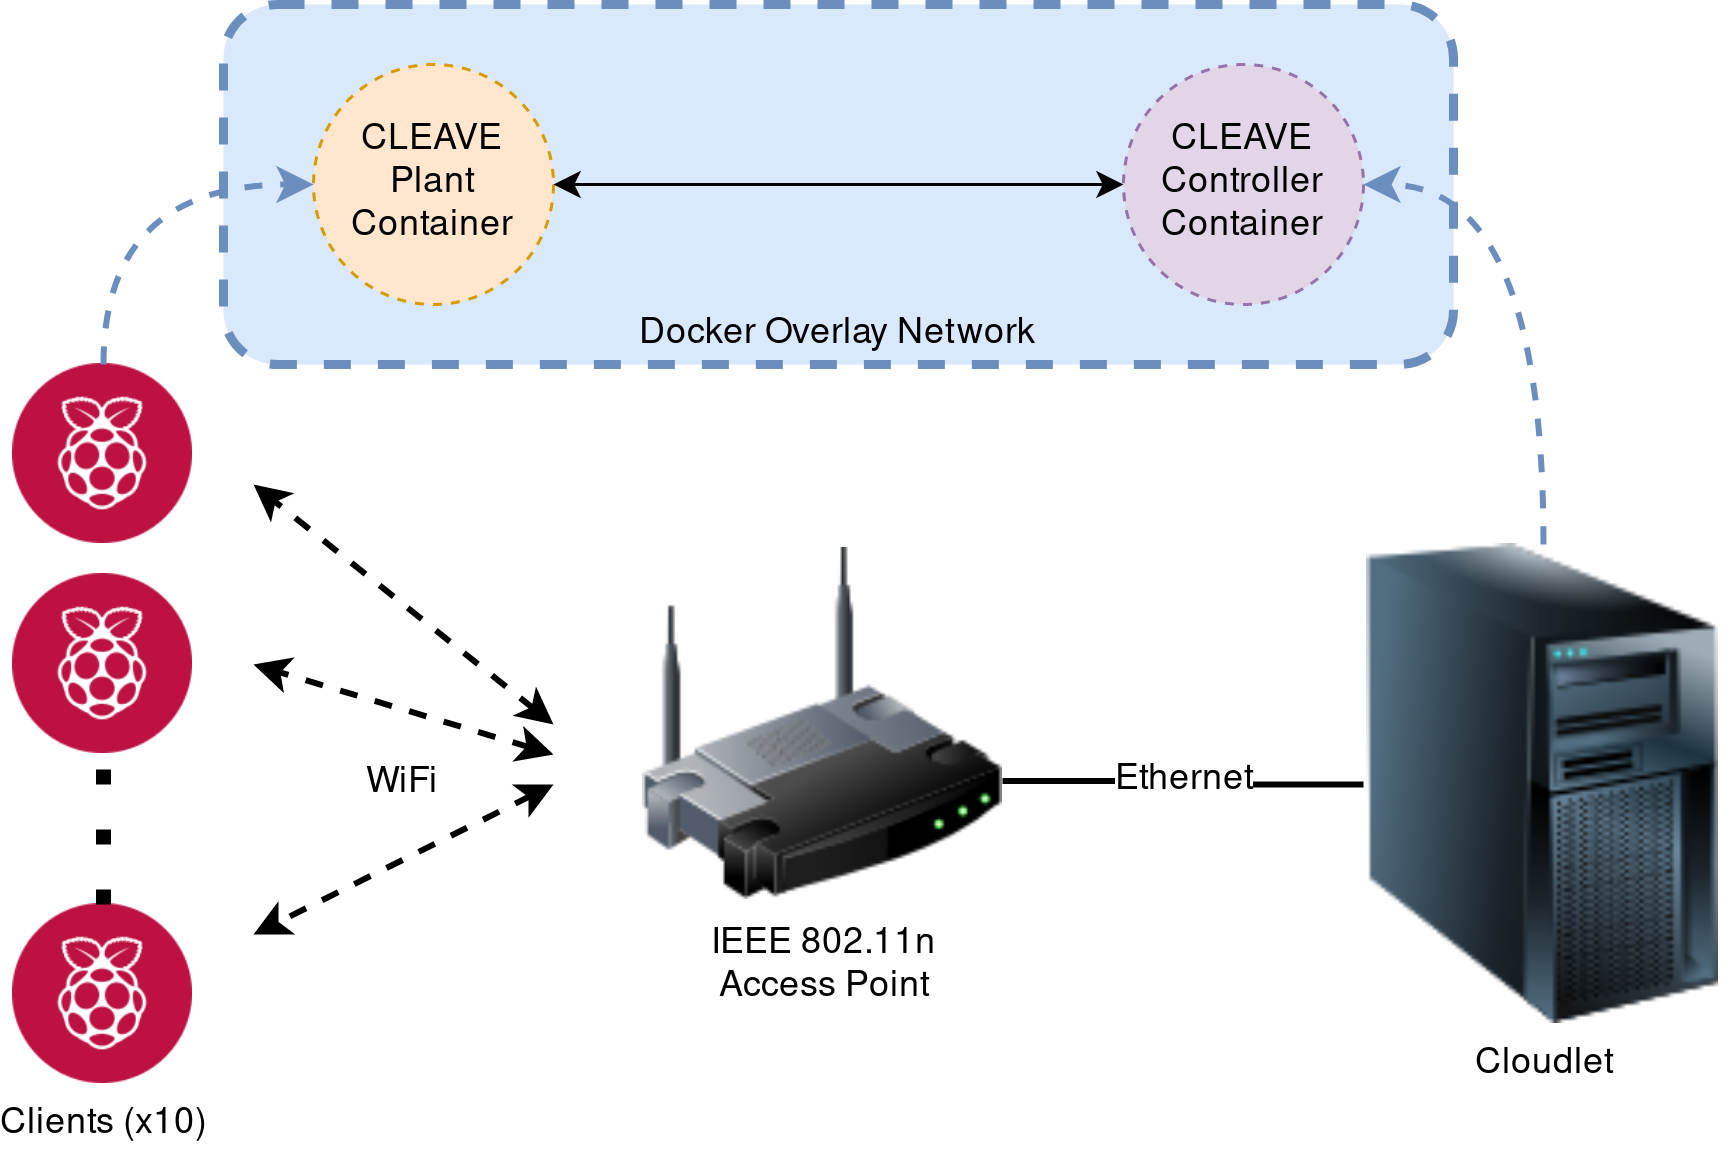
\includegraphics[width=.95\columnwidth]{images/CLEAVE_experiment_setup}
    \caption{
        The setup used for our experimentation. 
        % Containerized versions of the core CLEAVE emulation components are deployed inside a Docker Swarm Overlay Network spanning \num{10} Raspberry Pi 4B clients connected to a single Cloudlet over an IEEE 802.11n \ac{AP}.
    }\label{fig:cleave:expsetup}
\end{figure}

The first step in our case study is to evaluate the baseline performance of the control system, both locally and over the network.
We configure \ac{CLEAVE} to run a single loop with both plant and controller co-located on the Edge server, and we also configure a separate setup with an identical loop executed over the wireless link.
For both of these setups, we execute a series of scenarios varying:
\begin{enumerate*}[itemjoin={{; }}, itemjoin*={{; and }}]
    \item the sampling rate of the Plant state, setting it to \SIlist[list-final-separator={, or }]{5;10;20;40;60}{\hertz}
    \item the responsiveness of the Controller, adding fixed delays of \SIlist[list-final-separator={, or }]{0;25;50}{\milli\second} after the processing of each sample.
\end{enumerate*}

We run repeated executions of each combination of these parameters at least \num{10} times, for both the networked and ``local-only'' setups.
Each execution lasts for \SI{5}{\minute}, during which we collect detailed data on both the state of the controlled system as well as on the data sent over the network.
After the initial \num{10} runs, we identify that setups with sampling rates of \SIlist{5;10}{\hertz} were consistently too unstable to consider, and disregard them in further analyses.
We further note that setups with \SI{0}{\milli\second} additional delay are always stable and thus also disregard them.
Remaining setups, i.e.\ sampling rates \( \geq \) \SI{20}{\hertz} and artificial delays \( \geq \) \SI{25}{\milli\second}, are repeated an additional \num{20} times for better statistical significance.

This repeated experimentation and data collection while ``zooming in'' on particular setups is facilitated by \ac{CLEAVE}'s design.
Scenarios are executed automatically in batches using a simple Python script which interacts with Docker through the widely adopted \emph{docker-py}\footnote{Docker SDK for Python: \url{https://docker-py.readthedocs.io/en/stable/}} library.
This is \ac{CLEAVE}'s first advantage over existing frameworks; it is designed with cloud and edge technology and paradigms in mind, making integration with existing systems convenient.

\begin{figure}[t]
    \centering
    \begin{subfigure}[t]{\columnwidth}
        \centering
        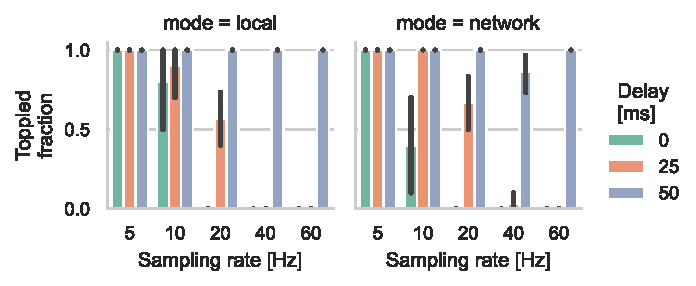
\includegraphics[width=\textwidth]{fixed_single_loop_toppled}
        \caption{Fraction of toppled plants.}\label{fig:single:topple}
    \end{subfigure}\\
    \begin{subfigure}[t]{\columnwidth}
        \centering
        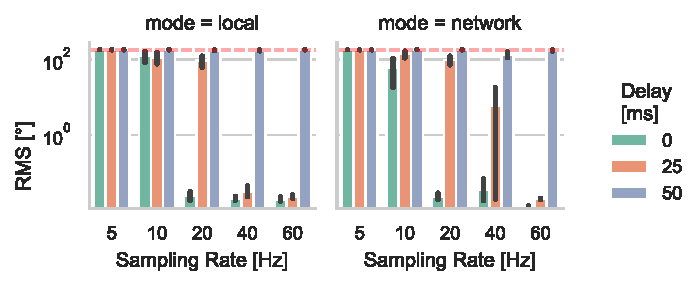
\includegraphics[width=\textwidth]{fixed_single_loop_rms}
        \caption{Mean angle \acs*{RMS}; red line indicates \( y = 180 \).}\label{fig:single:rms}
    \end{subfigure}\\
    \begin{subfigure}[t]{\columnwidth}
        \centering
        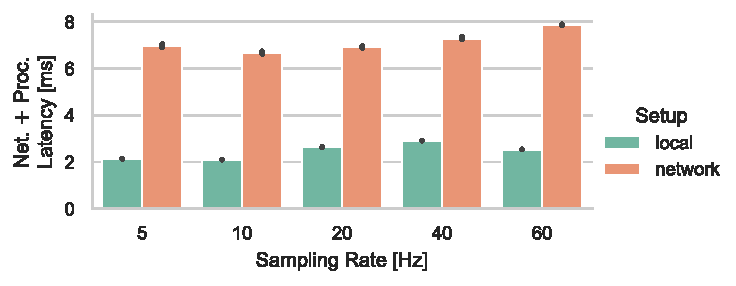
\includegraphics[width=\textwidth]{fixed_single_loop_rtts}
        \caption{
            Mean \acsp*{RTT}.
        }\label{fig:single:rtt}
    \end{subfigure}%
    \caption[caption]{
        Baseline results.
        Error bars indicate \SI{95}{\percent} \acp{CI}.
        }%
    \label{fig:single}
\end{figure}

\cref{fig:single} shows a summary of the results relating to the single-loop scenarios:
\cref{fig:single:topple} shows the fraction of plants that toppled in each scenario, and \cref{fig:single:rms} shows the average \ac{RMS} for the absolute pendula angles.
\cref{fig:single:rtt} shows average latency due to network and processing (excluding synthetic delays) for both single-loop scenarios.
Packet losses were below \SI{0.2}{\percent} for all parametrizations of the single-loop scenario over the network, and \SI{0}{\percent} for all parametrizations of the local-only setup.

As expected, higher sampling rates tend to correlate with better quality of control; at higher sampling rates the system was able to reach stability at higher \acp{RTT}.
These initial results already hint at interesting consequences for such an edge-bound \ac{NCS} deployment.
For instance, it is clear from \cref{fig:single:topple,fig:single:rms} that network delays can, to a certain extent, be compensated for by increasing the sampling rate of the system.
A corollary of this is, conversely, that at lower network latencies \acp{NCS} are able to stabilize at lower sampling rates.
Adaptive sampling might thus be a viable method for optimizing resource utilization.

Once baselines for single loops in the use case scenario have been established, we can proceed to studying the interaction between the \acp{NCS} and the video-streaming applications.
We deploy \num{6} control loops on the experimental setup depicted in \cref{fig:cleave:expsetup}.
On the remaining \num{4} clients we run the \emph{iperf3}\footnote{iperf3: \url{https://iperf.fr/}} traffic load generator, each generating \SI[per-mode=symbol]{6.5}{\mega\bit\per\second} of uplink \ac{UDP} traffic.
This emulates the load generated on the network by \SI{1080}{p} Full-HD video streaming, originating from the clients and terminating in the cloudlet.
Based on the baseline results, we execute setups with \ac{NCS} plant sampling rates of \SIlist{20;40;60}{\hertz}.
Each sampling rate configuration is run for \SI{5}{\minute}, and then repeated \num{30} times to obtain statistical significance.
Once again, repetitions of this scenario are executed automatically in batches using a simple Python script and \emph{docker-py}.

\begin{figure}[t]
    \centering
    \begin{subfigure}[h]{.22\textwidth}
        \centering
        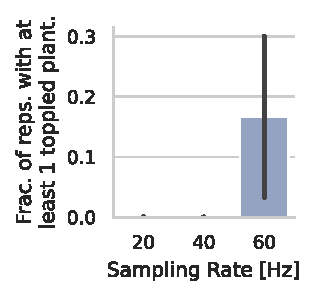
\includegraphics[width=\textwidth]{fixed_video_topple_frac}
        \caption{Toppled plants.}\label{fig:video:toppled}
    \end{subfigure}%
    \hfill%
    \begin{subfigure}[h]{.22\textwidth}
        \centering
        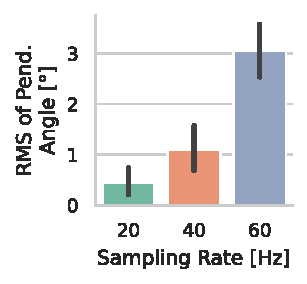
\includegraphics[width=\textwidth]{fixed_video_angle_rms}
        \caption{Angle \ac{RMS}.}\label{fig:video:rms}
    \end{subfigure}\\
    \begin{subfigure}[h]{.22\textwidth}
        \centering
        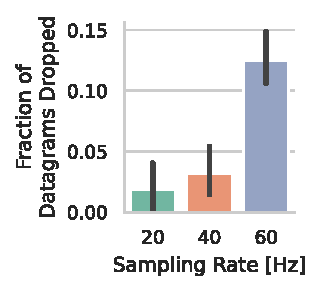
\includegraphics[width=\textwidth]{fixed_video_drop_frac}
        \caption{Packet losses.}\label{fig:video:drop}
    \end{subfigure}%
    \hfill%
    \begin{subfigure}[h]{.22\textwidth}
        \centering
        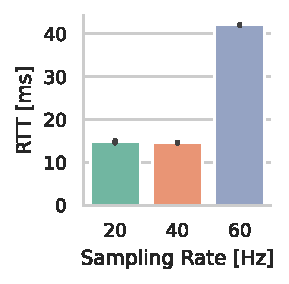
\includegraphics[width=\textwidth]{fixed_video_rtt}
        \caption{\acsp{RTT}.}\label{fig:video:rtt}
    \end{subfigure}%
    \caption{
        Multi-loop, resource-constrained setup results.
        Error bars indicate \SI{95}{\percent} \acp{CI} in all plots.
    }\label{fig:video:results}
\end{figure}

\cref{fig:video:results} shows a summary of the results obtained.
\cref{fig:video:toppled} shows the fraction of repetitions of each setup in which \emph{at least} one plant failed to maintain stability and toppled.
\cref{fig:video:rms} shows the \ac{RMS} for the pendulum angles for each setup, only considering data from plants that did not topple.
\cref{fig:video:drop} shows the fraction of \ac{UDP} datagrams dropped, averaged over all plants and repetitions per setup.
\cref{fig:video:rtt} shows the measured end-to-end plant-side \ac{RTT}, averaged over all plants and repetitions per setup.

These results are interesting in their counter-intuitiveness compared to the single-loop baseline results.
While the baselines might lead us to think that higher sampling rates are always better for the stability of control systems, \cref{fig:video:toppled,fig:video:rms} show this not to be the case for \ac{NCS} in resource-constrained scenarios.
\SI{60}{\hertz} was the least stable configuration, with at least one pendulum toppling in around \SI{16}{\percent} of the repetitions, and mean pendulum angle \ac{RMS} circa \num{3} times that of the \SI{40}{\hertz} scenario.
\SI{40}{\hertz} was in turn the second worst configuration --- although it presented no toppled pendula, average angle \ac{RMS} doubled that of the \SI{20}{\hertz} setup.

\cref{fig:video:drop,fig:video:rtt} explains these behaviors.
Whereas both the \SIlist{20;40}{\hertz} setups show losses well below \SI{5}{\percent}, the \SI{60}{\hertz} scenario shows an average of around \SI{13}{\percent} of datagrams lost.
The differences in \acp{RTT} results are equally telling; \acp{RTT} for the \SI{60}{\hertz} setup were on average approx.\ \num{3} times those for the \SIlist{20;40}{\hertz} setups.
These results stem from the contention for network resources, and hint at important trade-offs system designers will have to take into consideration when designing and developing \acp{NCS} for deployment on the Edge.
The Edge will be \emph{multi-tenant} and \emph{multi-instance}. 
\ac{NCS} deployments will have to be designed with shared resources in mind, and given the complexity of these systems, experimental tools like \ac{CLEAVE} will be key for their succesful adoption and massification.

\section{Conclusion}\label{sec:conclusion}

The issue of repeatable and scalable benchmarks has been largely glossed over in \ac{NCS} literature, as existing experimental research studies tend to implement \emph{ad-hoc} solutions.

In this work, we aimed to tackle this issue through a fully software-based framework for repeatable, reproducible, and easily scalable \ac{NCS} benchmarking with a particular focus on edge deployment.
We argue our approach, \ac{CLEAVE}, embodies a better solution than previous work for a number of reasons:
\begin{enumerate}
    \item Compared to fully physical approaches, such as those used in\ \cite{Baumann2018LowPower} and\ \cite{Cuenca2019UAV}, our approach allows for greater flexibility and scalability.
    The aforementioned approaches rely on specialized and sometimes entirely custom-built physical platforms, and although flexible and cheap approaches such as Zoppi \emph{et al.'s} --- which uses a LEGO-based physical plant --- exist, these still do not reach the level of flexibility afforded by a fully software-based framework. 
    Experimenters still need copies of the hardware, making anything other than small-scale setups unfeasible.
    In contrast, our approach requires only general-purpose computing platforms, and can be employed by basically anyone with access to a computer.
    Scalable deployments can in turn easily and cheaply be set up using single-board computers and/or virtual cloud instances.
    \item When compared to simulated approaches such as\ \cite{Ma2019DynamicSched}, \ac{CLEAVE} provides a higher level of realism, in particular with regards to the network segment of the system.
    \item Finally, although it shares much in common with previous emulated approaches such as the one employed in\ \cite{Wang2020VoltageControl}, \ac{CLEAVE} has an advantage by specifically targeting a general-purpose approach using industry-standard, cloud- and edge-native tools and software.
    The tool can easily be deployed and scaled using widely-used frameworks such as Docker Swarm and Kubernetes.
\end{enumerate}

We validate the utility of this tool through an example use case approximating a proposed edge deployment of inverted pendula control loops co-located with video analytics services.
We argue such a use case represents a realistic scenario and appropriate benchmark for the tool, since
\begin{enumerate*}[itemjoin={{; }}, itemjoin*={{; and }}]
    \item the inverted pendulum plant is ubiquitous in \ac{NCS} research
    \item similar setups exist in real-world industrial use
    \item video analytics has long been proposed as a ``killer app'' for edge computing.
\end{enumerate*}
Our results showcase the ability of the framework to extract relevant metrics relating to the stability of the control system, as well as on the performance of the underlying network link.
We believe \ac{CLEAVE} represents an important step towards enabling inexpensive and low-complexity scalable research for real-world deployment of edge-bound \acp{NCS}.

There is still, however, work to be done.
We are extending the number of plant and controller implementations on the framework, with the goal of creating an open library of \acp{NCS} to share with the community.
At the moment, the interactions of \ac{CLEAVE} and tools such as Docker are still quite superficial.
Our goal is to achieve a much tighter integration, e.g.\ by providing the toolkit as pre-packaged container images.
Finally, the validity of the results obtained by the framework will have to be verified through more thorough, realistic scenarios than what we have been able to show in this work.
In particular, we intend to perform large-scale experimentation targetting 5G cellular deployments, as this technology is set to become the backbone of edge networks in the near future.

%%%%%%%%%%%%%%%%%%%%%%%%%%%%%%%%%%%%%%%
%%%%%%%% ACKNOWLEDGMENT %%%%%%%%%%%%%%%
%%%%%%%%%%%%%%%%%%%%%%%%%%%%%%%%%%%%%%%
\chapter{Acknowledgements}
\epigraph{La educación es, tal vez, la forma más alta de buscar a Dios.}{\emph{Gabriela Mistral}}
\glsresetall%

There are many, many people I owe gratitude to for making this dissertation possible.
I would like to begin by thanking my supervisor, Prof. James Gross.
This dissertation would not have been possible without his guidance and motivation during this long process.
His supervision opened doors that I had never imagined would open for me, and his dry German humor has certainly helped cheer me up whenever I was overwhelmed by some deadline.
Above all, I would like to thank James for his patience and understanding whenever I encountered difficulties, and for the flexibility he has afforded me in completing this Ph.D.

I would like to express my deepest gratitude to Prof. Mahadev ``Satya'' Satyanarayanan, for welcoming me repeatedly, over long periods of time, as a visiting researcher at \gls{CMU}.
Likewise, I'm deeply indebted to Prof. Roberta ``Bobby'' Klatzky of \gls{CMU} for the many helpful and insightful discussions, for introducing me to the field of Human-Computer Interaction, and for always greeting me with a warm smile.
Both Satya's and Bobby's tremendous experience and generosity have been invaluable, and their guidance and advice have certainly shaped my work for the better.

I would also like to thank everybody involved with the defense of this thesis.
I am very grateful to Prof. Yu Xiao of Aalto University, for agreeing to act as my dissertation opponent.
My dissertation defense will certainly benefit greatly from her expertise and insights.
I would like to extend my sincere thanks to my grading committe, consisting of Prof. Ana Aguiar (Universidade do Porto), Prof. Per Gunningberg (Uppsala Universitet), and Prof. Klaus Wehrle (\gls{RWTH}), for investing time and effort into reading and grading this dissertation.
Special thanks also go to Prof. Markus Flierl of \pgls{KTH} for advance-reviewing this dissertation, and to Prof. Mats Bengtsson, also of \pgls{KTH}, for agreeing to act as chairperson for the defense.

Moreover, I extend my thanks to my co-authors and colleagues.
To Samie Mostafavi, Vishnu N. Moothedath, and Neelabhro Roy at \pgls{KTH}, for always being willing to engage in interesting discussions, but also for generally being fun to be around.
And to Dr. Jaya Prakash (IMDEA Networks Institute), Dr. Junjue Wang (\gls{CMU}), and Dr. Padmanabhan ``Babu'' Pillai (\gls{CMU}) for enriching my research with their interesting insights.

I am very lucky and grateful that I got to stay at both \pgls{KTH} and \gls{CMU}, and I would like to thank everyone who made these spaces welcoming and engaging.
A big thank you goes out to my colleagues (both current and former) at the division of \gls{ISE} for all those fun lunches at Restaurang Q, Cypern, and SysterOBror over the years, which always helped to break the monotony of the days.
This includes but is not limited to Samie, Vishnu, Neel, Sahar, Antonios, Germán, Boules, Baptiste, Håkan, Pol, Marie, Wendi, and Sebastian.
I would additionally like to extend a special thank you to Dr. Sebastian Schiessl, for ``taking me under his wing'' when I first arrived at \gls{ISE} and acting as a sort of mentor during my first moths.
Likewise, I extend my gratitute to Gerd Fransson, for greeting me with a huge smile every morning the years our offices faced each other and cheering up my days with her wholesome energy.
I also thank Prof. Joakim Jaldén for giving me the opportunity to act as his teaching assistant.
Another big thank you goes out to everyone (current and former) at Satya's group at \gls{CMU}, for always welcoming me with open arms and treating me like one of them whenever I was visiting.
This includes but is not limited to Junjue, Tom, Roger, Shilpa, Jan, Edmond, Jim, Babu, and Zhuo.
I will always remember our Monday morning talks and Friday lunch outings dearly.

Furthermore, I would like to extend my sincere thanks to Prof. Sandra Céspedes, of Universidad de Chile and Concordia University, for her guidance and urging to embark on this journey towards a Ph.D., and for always being willing to offer help and advice.
Likewise, I'd like to thank Prof. Javier Bustos, of Universidad de Chile and NIC Chile Research Labs, for giving me the opportunity many years ago to first get into distributed systems research.
Also, I'd like to extend my gratitude to Prof. José Miguel Piquer, of Universidad de Chile, for taking me as his ``long-distance'' teaching assistant and allowing me to give back to my \emph{alma mater} from across the ocean.
A very special thanks goes out to Prof. Jérémy Barbay of Universidad de Chile and Universidad de Concepción, for being both a mentor and a friend since the day I took his course on Android programming as an undergraduate student.
I am deeply appreciative of the fact that although our interactions these last few years have been sporadic at best, I can always reach out to him for help and advice when I need them.

\medskip

This dissertation would not have been possible without the help and support of my family.
First and foremost, I would like to thank the love of my life and wife~\footnote{\emph{Future-wife} at the time of writing, but \emph{wife} at the time of the defense of this thesis!}, Andresa.
I could not have done this without her companionship and love.
I am eternally grateful for her unconditional support over difficult periods of time and over tremendous distances while we were living apart, and for making every day we spend together amazing.

I am also deeply grateful to my parents, Gabriel and Valeria, for always encouraging my curiosity and my drive to learn and discover.
They have been my rocks, my pillars, since the day I was born, and I am proud to be their son.
A big thank you goes out to my sister, Paola, as well.
Although we sometimes get on each other's nerves, she has always been there for me and supported me, and I could not have asked for a better sister.
Likewise, I extend my deepest gratitude to everyone in my immediate and extended family who have given me support and love over the years, including but not limited to my paternal grandparents, Manuel and María Yolanda, my maternal grandparents, Caupolicán and María Aura, my uncle Mauricio, his wife Marylen, their daughter Amanda, and everybody else.
I would like to make a special mention to my late grandfather, Caupolicán ``Poli'' Muñoz, who always inspired and fanned the flames of academic curiosity in me.
I hope he would have been proud seeing how far I have come.
Another special mention goes to my uncle Manuel, who graciously took me in and gave me a place to stay at the first few months of my Ph.D. studies.

I would also like to thank all of my friends who have made this long, ardous journey more amenable.
I would particularly like to thank everyone I met through Tartan Salsa, including, but not limited to, Andresa, Jennifer, Alyson, Kuai-Kuai, Carmen, Moataz and Nora, Eric, and many others.
They made Pittsburgh feel like home, even before I finally moved there permanently in 2022.
I also want to thank Ann-Charlotte in Stockholm, for always being so kind, so considerate, and so much fun to be around.
Further, I am deeply grateful to my friends in Chile who have remained a source of support, even though we only get to see each other once a year when I visit.
This includes, but is not limited to, Juan Pablo, Fernanda, Diego, Camila, George, Patricio, Kevin, Pablo, and many others.
Yet another special mention goes to Diego's family, who have always treated me as one of their own.

Finally, I would be remiss in not mentioning my pets and animal friends who have provided me with love and warmth during these years.
I thank my dogs, Aros and Skatt, who I sadly had to leave behind in Chile with my sister, but who still greet me with enthusiastically wagging tails whenever I visit.
And I thank my cats, Mochi and Tiramisú, who, although have only been in my life for about a year, have sweetened and made much more bearable the long days and nights I have spent writing this dissertation.

\bigskip

\noindent{}Manuel Olguín Muñoz\\
Pittsburgh, May 2023
% \printbibliography{}
% \printbibitembibliography{}

\begin{thebibliography}{99}
  %
  \bibitem{Rajkumar2010CPS}
  Ragunathan Rajkumar et al. “Cyber-physical systems: The next computing revolution”. In: \emph{Proceedings of the Design Automation Conference}. 2010, pp. 731–736.
  %
  \bibitem{Satya2017Emergence}
  Mahadev Satyanarayanan. “The Emergence of Edge Computing”. In: \emph{Computer} 50.1 (2017), pp. 30–39.
  %
  \bibitem{Gupta2010NCSOverview}
  Rachana Ashok Gupta and Mo-Yuen Chow. “Networked Control System: Overview and Research Trends”. In: \emph{IEEE Transactions on Industrial Electronics} 57.7 (2010), pp. 2527–2535. %
  \bibitem{Wan2020Efficient}
  Shaohua Wan et al. “Efficient computation offloading for {Internet of Vehicles} in edge computing-assisted 5G networks”. In: \emph{The Journal of Supercomputing} 76.4 (2020), pp. 2518–2547. %
  \bibitem{Baumann2018LowPower}
  Dominik Baumann et al. “Evaluating Low-Power Wireless Cyber-Physical Systems”. In: \emph{Proceedings of the First IEEE Workshop on Benchmarking Cyber-Physical Networks and Systems (CPSBench’18)}. 2018, pp. 13–18.
  %
  \bibitem{Cuenca2019UAV}
  Ángel Cuenca et al. “Periodic Event-Triggered Sampling and Dual-Rate Control for a Wireless Networked Control System With Applications to {UAVs}”. In: \emph{IEEE Transactions on Industrial Electronics} 66.4 (2019), pp. 3157–3166.
  %
  \bibitem{Ma2019DynamicSched}
  Yehan Ma et al. “Optimal Dynamic Scheduling of Wireless Networked Control Systems”. In: \emph{Proceedings of the 10th ACM/IEEE International Conference on Cyber-Physical Systems}. Association for Computing Machinery, 2019, 77–86.
  %
  \bibitem{Wang2020VoltageControl}
  Yu Wang et al. “Inverter-Based Voltage Control of Distribution Networks: A Three-Level Coordinated Method and Power Hardware-in-the-Loop Validation”. In: \emph{IEEE Transactions on Sustainable Energy} 11.4 (2020), pp. 2380–2391.
  %
  \bibitem{Natale2004InvPendEthernet}
  O.R. Natale et al. “Inverted pendulum stabilization through the {Ethernet} network, performance analysis”. In: \emph{Proceedings of the 2004 American Control Conference}. Vol. 6. 2004, 4909–4914 vol.6.
  %
  \bibitem{Zoppi2020NCSBench}
  Samuele Zoppi et al. “{NCSbench}: Reproducible Benchmarking Platform for Networked Control Systems”. In: \emph{Proceedings of the {17th} IEEE Annual Consumer Communications Networking Conference (CCNC’20)}. 2020, pp. 1–9.
  %
  \bibitem{Olguin2019EdgeDroid}
  Manuel Osvaldo J. Olguín Muñoz et al. “{EdgeDroid: An Experimental Approach to Benchmarking Human-in-the-Loop Applications}”. In: \emph{Proceedings of the 20th International Workshop on Mobile Computing Systems and Applications}. ACM, 2019, pp. 93–98.
  %
  \bibitem{Ananthanarayanan2017Analytics}
  Ganesh Ananthanarayanan et al. “Real-Time Video Analytics: The Killer App for Edge Computing”. In: \emph{Computer} 50.10 (2017), pp. 58–67.
  %
  \bibitem{Yi2017Analytics}
  Shanhe Yi et al. “LAVEA: Latency-Aware Video Analytics on Edge Computing Platform”. In: \emph{Proceedings of the Second ACM/IEEE Symposium on Edge Computing}. Association for Computing Machinery, 2017.
  %
  \bibitem{Wang2018Analytics}
  Junjue Wang et al. “Bandwidth-Efficient Live Video Analytics for Drones Via Edge Computing”. In: \emph{Proceedings of the Third IEEE/ACM Symposium on Edge Computing (SEC)}. Association for Computing Machinery, 2018, pp. 159–173.
\end{thebibliography}

\end{document}